
In this first exercise we implemented the regression of a function in one-dimensional case, for example: the quadratic function
\[y = x^2,\  \forall x\in[0,1]\]
Vengono definite:

\begin{itemize}

	\item Function to be rebuilt
	\item The number of samples
	\item The samples disturbed by the Gaussian additive noise
	\item The variance of the noise
	\item The degree of the polynomial regressor

\end{itemize}

\begin{figure}[h]
	\centering
	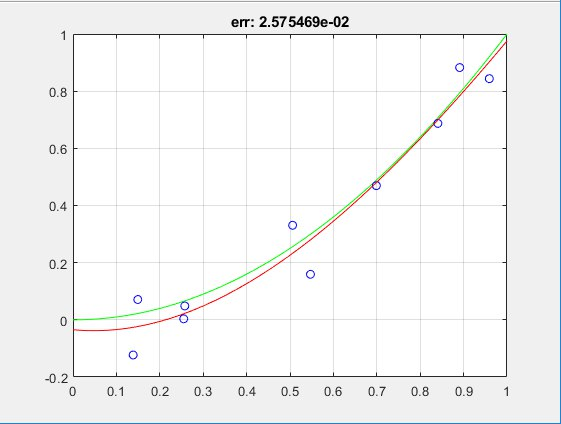
\includegraphics[width=0.5\textwidth]{regression_function.png}
	\caption{Regression Function}
	\label{fig:regression function}
\end{figure}

Figure \ref{fig:regression function} Regression function of a quadratic function\\
Starting from this first test, we notice that increasing the complexity of the polynomial too much produce a great loss of precision in the reconstruction.
It's therefore necessary to evaluate the variation of reconstruction, by changing $ n $ (Number of samples), $ p $ (Degree of the polynomial regressor) and $ \sigma $ (Noise variance).
So the error is calculated between $ YT $ (True function) and $ YP $ (Prediction function) and plotted in the graph. \\
Now we notice that in order to make the measurement of error more precise, it's better to repeat the experiment a sufficiently high number of times, for example, we make 30 repetitions of the prediction.

\begin{figure}[!tbp]
	\centering
	\subfloat[Error by varying n and p (from 0 to 5)]{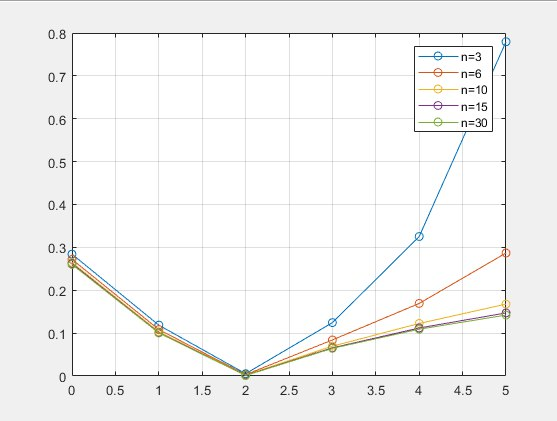
\includegraphics[width=0.45\textwidth]{error_varying_n_p.png}\label{fig:error by varying n and p}}
	\hfill
	\subfloat[Error by varying n and p (from 0 to 3)]{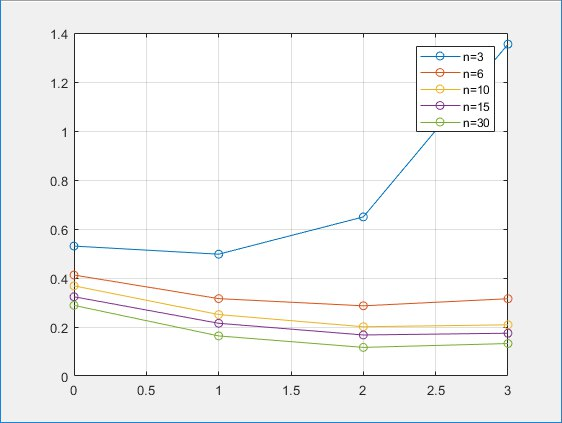
\includegraphics[width=0.45\textwidth]{error_varying_n_p2.png}\label{fig:error by varying n and p}}
	\caption{Comparing error with different values of p}
\end{figure}

\begin{figure}[!tbp]
	\centering
	\subfloat[Error by varying n and p (from 0 to 5)]{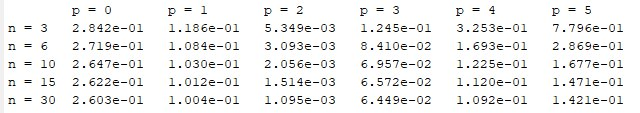
\includegraphics[width=0.5\textwidth]{table_error_varying_n_p.png}\label{fig:error by varying n and p}}
	\hfill
	\subfloat[Error by varying n and p (from 0 to 3)]{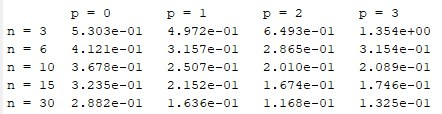
\includegraphics[width=0.4\textwidth]{table_error_varying_n_p2.png}\label{fig:error by varying n and p}}
	\caption{Comparing error with different values of p}
\end{figure}

We performed tests with some values of $ n $ and $ p $, from which it becomes clear how the error always maintains the same trend.
In particular, observing the error plots, it's evident that the maximum degree of precision is obtained for $p$ values around the degree of the original function. Obviously, using a second degree polynomial the error is minimal since the function to be reconstructed is a parabola.
Utilizing a large number of samples $n$, in general, also increases accuracy, while an increase of $p$ results in a loss of precision.
It's evident that the variation of the error between one execution of the exercise and the other is minimal for the values greater than n.
While using a small number of samples $n$, it's better to use low-grade polynomials, since an excessive number of degrees of freedom results in an attempt of the regression function to pass for each sample, making the reconstruction less precise, in particular in presence of a lot of noise, as it will try to pass for the samples even if noisy.










